\subsection{Design Goals}

We want to provide an architecture for Web data processing that is based on unified treatment of data on annotation and processing side
and that allows the backend machinery to access all information contained in a Web page, including how it is presented to a Web surfer.

\subsection{Requirements}

\begin{description}

\item[Flexibility]
The system should be open enough to allow customization of every part, but also specifically provide stable interfaces for more common tasks to allow for modularization.

\item[Stability]
We need a stable http data source that is independent of the original Website, including any dependencies such as images, stylesheets or scripts.

\item[Automaticity]
Backend processing should run without requiring any kind of human interaction.

\item[Replicability]
Computations carried out on Web pages' representation must be replicable accross systems, including any user-side processing.

\item[Quantity]
Corpus size should not influence the performance of the system and total processing time should grow linearly with the corpus.

\item[Usability]
Usability of the annotators side is of paramount importance, so we should stay as close as possible to the everyday Web experience.
We also need to provide tools for learning how to use the annotation tool and how to annotate Web pages.

\end{description}

\subsection{Core Architecture}

To address these requirements, we developed an abstract architecture, a simplified version of which is depicted in figure \ref{f:arch}.
We will outline the rationale for the basic design decisions below.


For rendering a Web page, an object tree is constructed from its HTML source code.
This tree can be traversed and its nodes inspected, modified, deleted and created through an API specified by the World Wide Web Consortium's (W3C) DOM Standard \cite{dom}.
It's most popular use case is client-side dynamic manipulation of Web pages, for visual effects and interactivity.
This is most commonly done by accessing the DOM through a JavaScript interpreter.
Essentially, a page's DOM tree allows access to all the information we set out to work on: structure, textual content and visual rendering data.
We therefore make it the sole interface between application and data.

While all browsers try to implement some part of the DOM standard (currently, version 3 is only partially implemented in most popular browsers), they vary greatly in their level of compliance as well as their ability to cope with non-standard compliant content.
This leads to structural and visual differences between different browsers rendering the same Web page.

Therefore, to guarantee \textit{replicability}, we require the same DOM engine to be used through the system.


To reach a maximal level of \textit{automaticity} and not to limit the \textit{quantity} of the data, it is important that data analysis can take place in a parallel fashion and does not require any kind of graphical interface, so it can e.g. be executed on server farms.
On the other hand we also need to be able to present pages within a browser to allow for user annotation.

Consequently, the same DOM engine needs to power a browser as well as a headless back-end application, with \textit{usability} being an important factor in the choice of a particular browser.


The annotation process, especially the order of presentation of pages, is controlled by a central Web server.
Thereby any number of concurrent annotators can be coordinated and submissions distributed equally across cropora.
All data, un-classified and user-submitted, is stored in a database attached to the Web server.
This setup allows the architecture to scale \textit{automatically} with user numbers under any usage pattern and submission \textit{quantity}.


\textit{Stability} of data sources is a major problem when dealing with Web data.
As we work on Web pages and the elements contained in them, simple HTML dumping is not an option.
Instead, we use a HTTP proxy to cache Web data used in our own storage.
By setting the server to grab content only upon first request and providing a option to turn off download of new data, we can create a closed system that does not change anymore once populated.


\begin{figure}
\jss{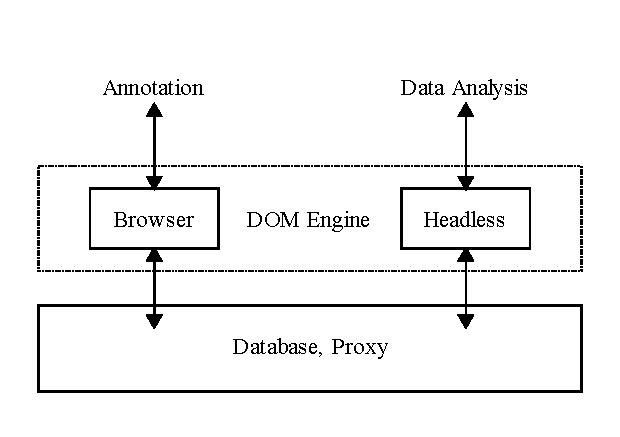
\includegraphics[width=0.4\textwidth]{arch}}
	{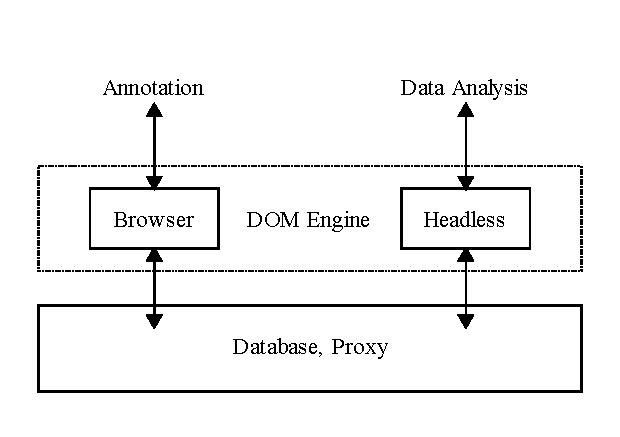
\includegraphics[width=0.8\textwidth]{arch}}
\caption{\label{f:arch}Basic {\KrdWrd} architecture: both users annotating corpus pages through their Web browser
and back-end applications working on the data run the same DOM engine.
	The central server delivers and stores annotation data and coordinates user submissions.}
\end{figure}


